\begin{figure}[H]
  \begin{center}
    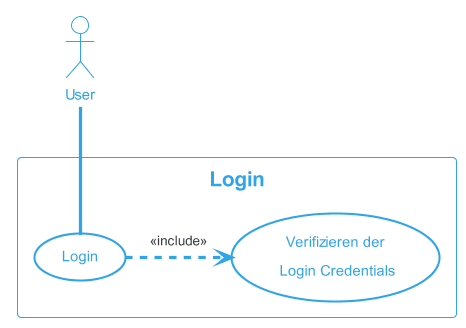
\includegraphics[width=0.6\linewidth]{content/diagrams/out/usecase/login/Login.png}
    \caption{UC-Login}
  \end{center}
  \label{login}
\end{figure}

\begin{table}[H]
  \newcolumntype{a}{>{\columncolor[HTML]{1EB6FF}}L}
  \centering
  \settowidth\tymin{\textbf{Kurzbeschreibung}}
  \setlength\extrarowheight{2pt}
  \begin{tabulary}{1.0\textwidth}{|a|m{12cm}|}
    \hline
    \textbf{Name}& Login\\
    \hline 
    \textbf{Kurzbeschreibung} & \\
    \hline
    \textbf{Beteiligte Aktoren} & \\
    \hline
    \textbf{Fachverantwortlicher} & \\
    \hline
    \textbf{Referenzen} & \\
    \hline
    \textbf{Vorbedingungen} & \\
    \hline
    \textbf{Nachbedingungen} & \\
    \hline
  \end{tabulary}
  \caption{UC-Login}
\end{table}

\begin{figure}[H]
  \begin{center}
    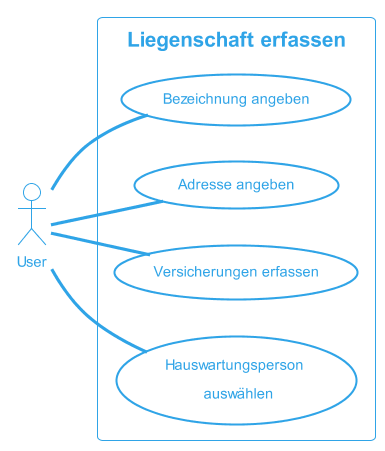
\includegraphics[width=0.4\linewidth]{content/diagrams/out/usecase/liegenschaftErfassen/LiegenschaftErfassen.png}
    \caption{Usecase Liegenschaft erfassen}
  \end{center}
  \label{Liegenschaft}
\end{figure}

\begin{table}[H]
  \newcolumntype{a}{>{\columncolor[HTML]{1EB6FF}}L}
  \centering
  \settowidth\tymin{\textbf{Kurzbeschreibung}}
  \setlength\extrarowheight{2pt}
  \begin{tabulary}{1.0\textwidth}{|a|m{12cm}|}
    \hline
    \textbf{Name}& Login\\
    \hline 
    \textbf{Kurzbeschreibung} & \\
    \hline
    \textbf{Beteiligte Aktoren} & \\
    \hline
    \textbf{Fachverantwortlicher} & \\
    \hline
    \textbf{Referenzen} & \\
    \hline
    \textbf{Vorbedingungen} & \\
    \hline
    \textbf{Nachbedingungen} & \\
    \hline
  \end{tabulary}
  \caption{UC-Login}
\end{table}

\begin{figure}[H]
  \begin{center}
    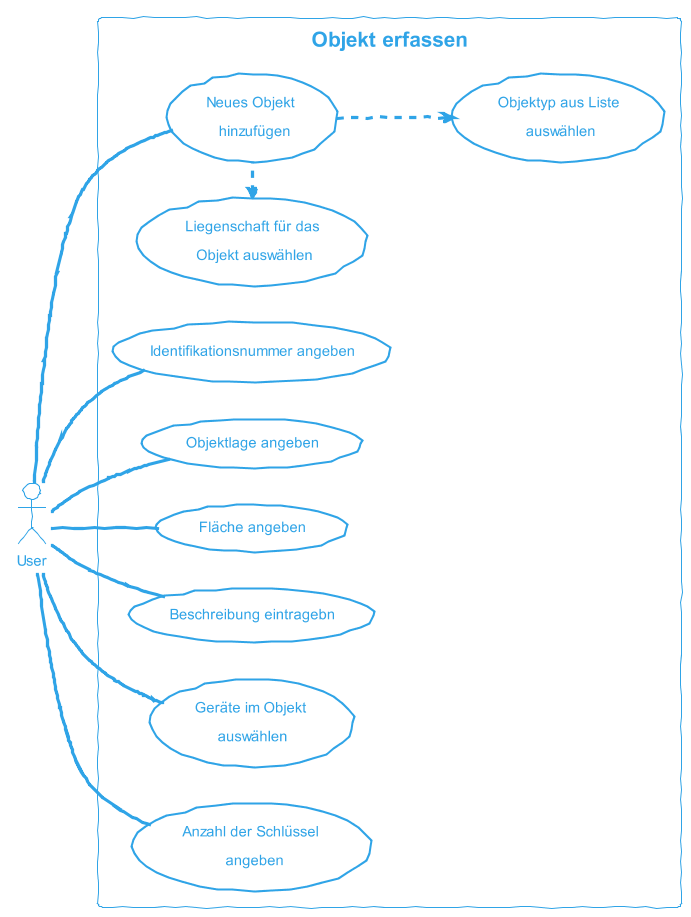
\includegraphics[width=0.8\linewidth]{content/diagrams/out/usecase/objektErfassen/ObjektErfassen.png}
    \caption{UC-Objekt Erfassen}
  \end{center}
  \label{objekt}
\end{figure}

\begin{table}[H]
  \newcolumntype{a}{>{\columncolor[HTML]{1EB6FF}}L}
  \centering
  \settowidth\tymin{\textbf{Kurzbeschreibung}}
  \setlength\extrarowheight{2pt}
  \begin{tabulary}{1.0\textwidth}{|a|m{12cm}|}
    \hline
    \textbf{Name}& Login\\
    \hline 
    \textbf{Kurzbeschreibung} & \\
    \hline
    \textbf{Beteiligte Aktoren} & \\
    \hline
    \textbf{Fachverantwortlicher} & \\
    \hline
    \textbf{Referenzen} & \\
    \hline
    \textbf{Vorbedingungen} & \\
    \hline
    \textbf{Nachbedingungen} & \\
    \hline
  \end{tabulary}
  \caption{UC-Login}
\end{table}

\begin{figure}[H]
  \begin{center}
    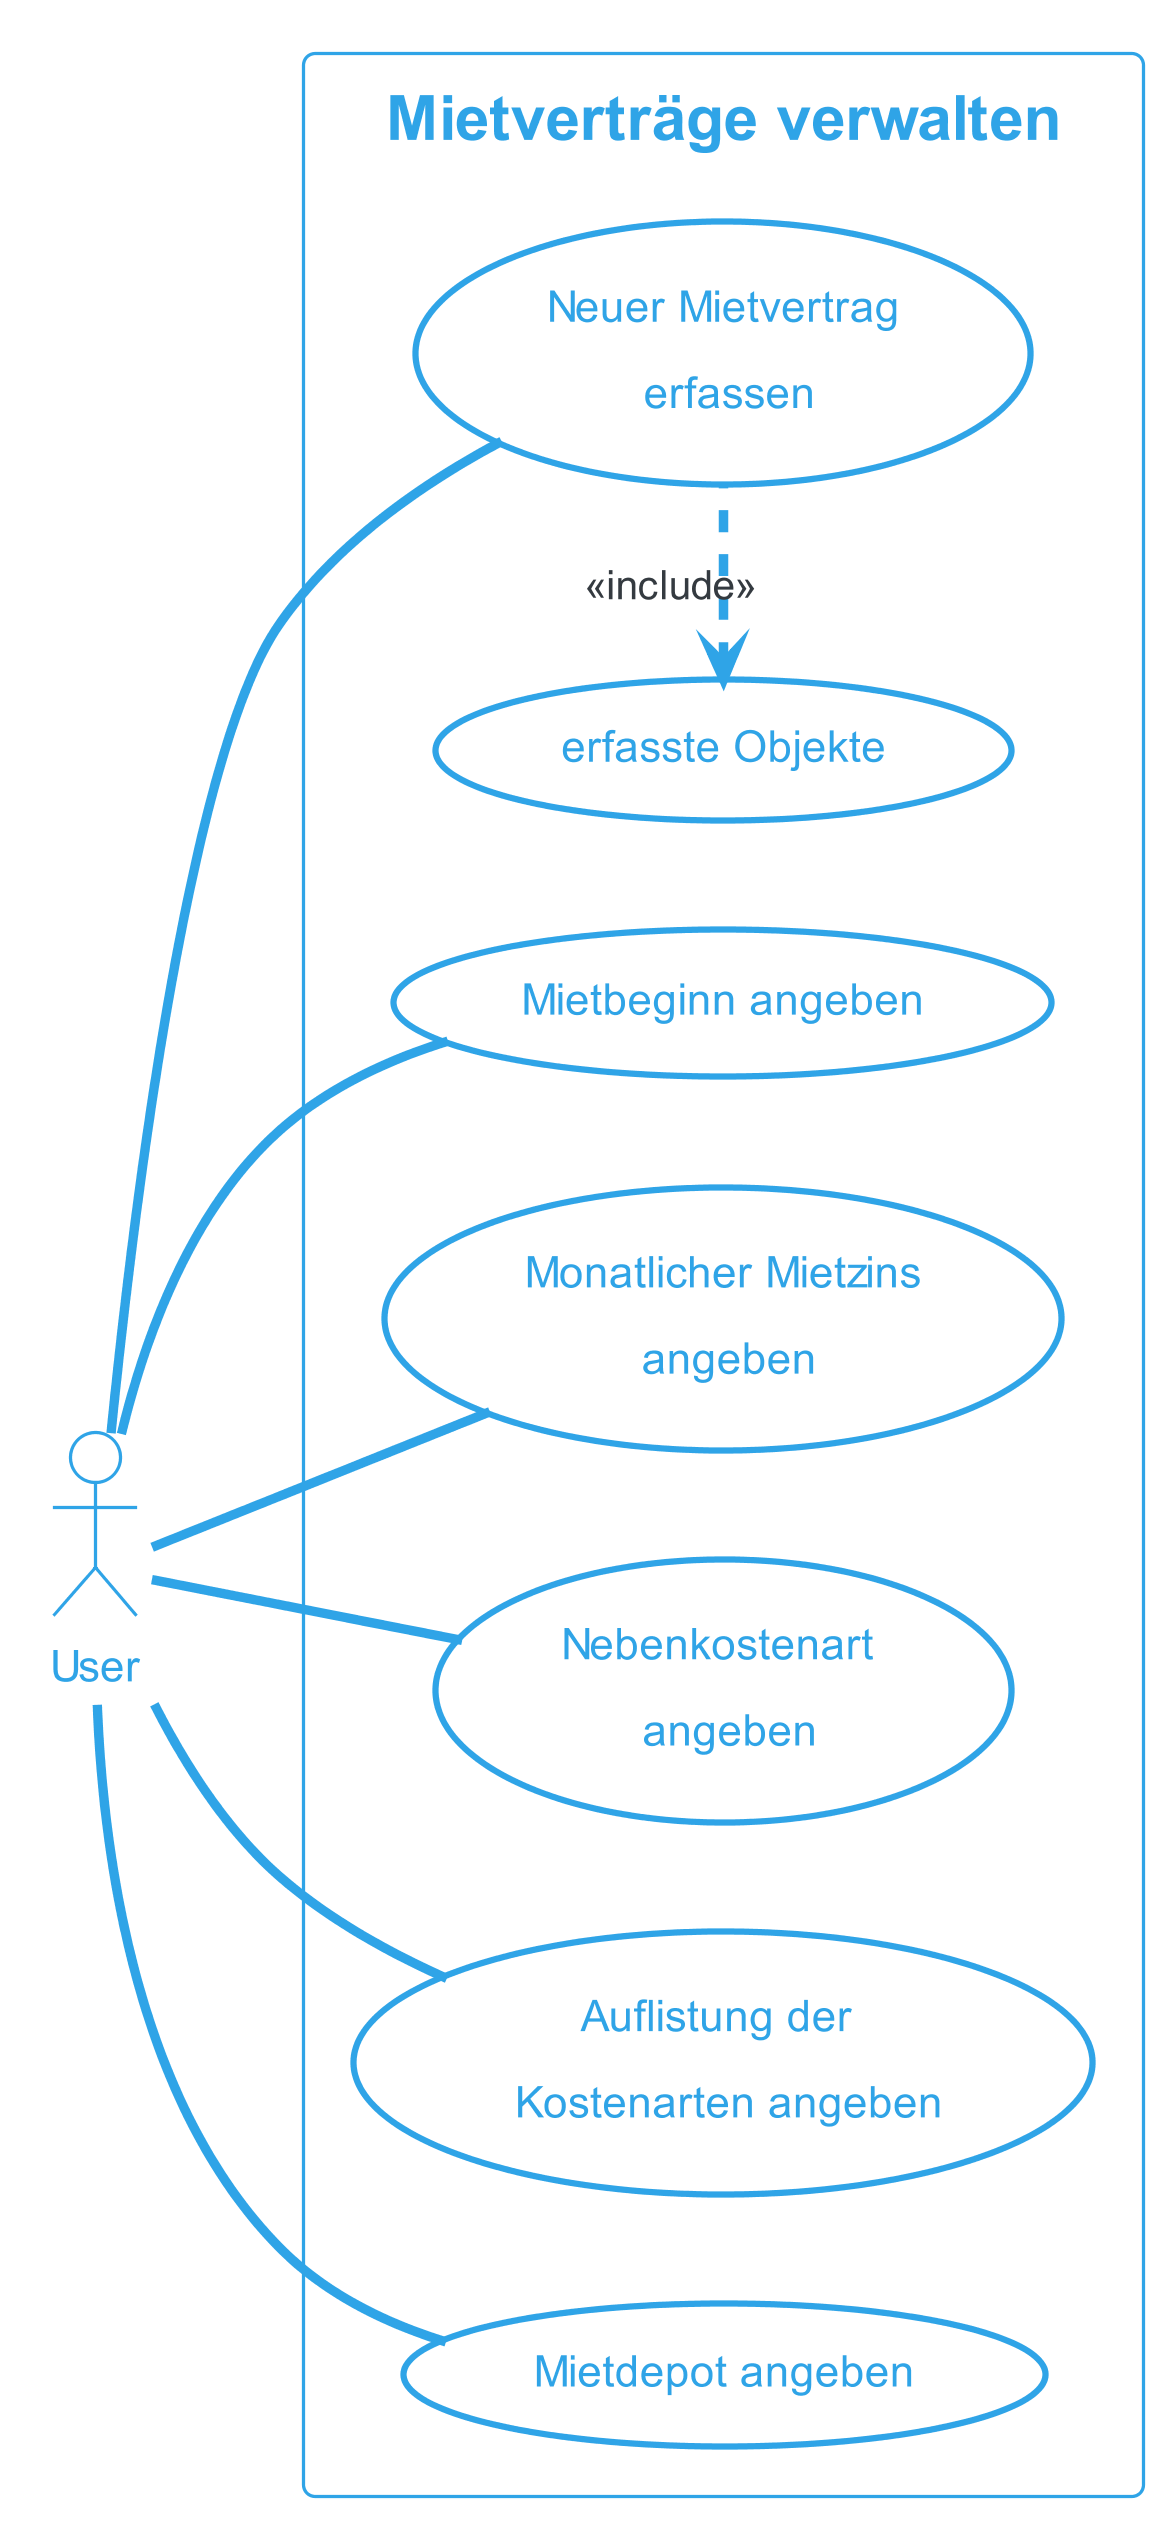
\includegraphics[width=0.45\linewidth]{content/diagrams/out/usecase/mietverträgeVerwalten/MietverträgeVerwalten.png}
    \caption{UC-Mietverträge Verwalten}
  \end{center}
  \label{MietvertraegeVerwalten}
\end{figure}

\begin{table}[H]
  \newcolumntype{a}{>{\columncolor[HTML]{1EB6FF}}L}
  \centering
  \settowidth\tymin{\textbf{Kurzbeschreibung}}
  \setlength\extrarowheight{2pt}
  \begin{tabulary}{1.0\textwidth}{|a|m{12cm}|}
    \hline
    \textbf{Name}& Login\\
    \hline 
    \textbf{Kurzbeschreibung} & \\
    \hline
    \textbf{Beteiligte Aktoren} & \\
    \hline
    \textbf{Fachverantwortlicher} & \\
    \hline
    \textbf{Referenzen} & \\
    \hline
    \textbf{Vorbedingungen} & \\
    \hline
    \textbf{Nachbedingungen} & \\
    \hline
  \end{tabulary}
  \caption{UC-Login}
\end{table}

\begin{figure}[H]
  \begin{center}
    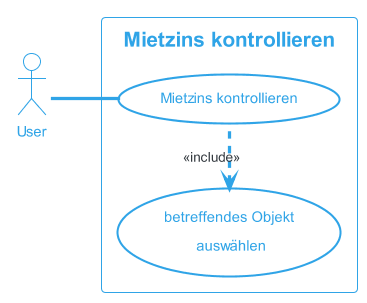
\includegraphics[width=0.4\linewidth]{content/diagrams/out/usecase/mietzinsKontrollieren/MietzinsKontrollieren.png}
    \caption{UC-Mietzins Kontrollieren}
  \end{center}
  \label{MietzinsKontrollieren}
\end{figure}

\begin{table}[H]
  \newcolumntype{a}{>{\columncolor[HTML]{1EB6FF}}L}
  \centering
  \settowidth\tymin{\textbf{Kurzbeschreibung}}
  \setlength\extrarowheight{2pt}
  \begin{tabulary}{1.0\textwidth}{|a|m{12cm}|}
    \hline
    \textbf{Name}& Login\\
    \hline 
    \textbf{Kurzbeschreibung} & \\
    \hline
    \textbf{Beteiligte Aktoren} & \\
    \hline
    \textbf{Fachverantwortlicher} & \\
    \hline
    \textbf{Referenzen} & \\
    \hline
    \textbf{Vorbedingungen} & \\
    \hline
    \textbf{Nachbedingungen} & \\
    \hline
  \end{tabulary}
  \caption{UC-Login}
\end{table}

\begin{figure}[H]
  \begin{center}
    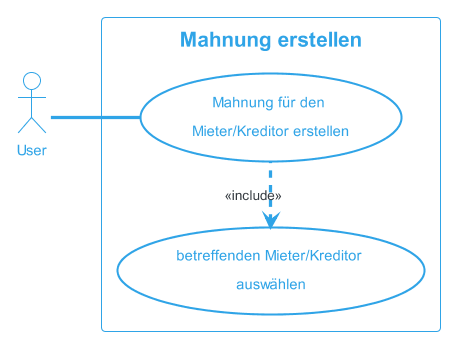
\includegraphics[width=0.4\linewidth]{content/diagrams/out/usecase/mahnungGenerieren/MahnungErstellen.png}
    \caption{UC-Mahnung Erstellen}
  \end{center}
  \label{mahnung}
\end{figure}

\begin{table}[H]
  \newcolumntype{a}{>{\columncolor[HTML]{1EB6FF}}L}
  \centering
  \settowidth\tymin{\textbf{Kurzbeschreibung}}
  \setlength\extrarowheight{2pt}
  \begin{tabulary}{1.0\textwidth}{|a|m{12cm}|}
    \hline
    \textbf{Name}& Login\\
    \hline 
    \textbf{Kurzbeschreibung} & \\
    \hline
    \textbf{Beteiligte Aktoren} & \\
    \hline
    \textbf{Fachverantwortlicher} & \\
    \hline
    \textbf{Referenzen} & \\
    \hline
    \textbf{Vorbedingungen} & \\
    \hline
    \textbf{Nachbedingungen} & \\
    \hline
  \end{tabulary}
  \caption{UC-Login}
\end{table}

\begin{figure}[H]
  \begin{center}
    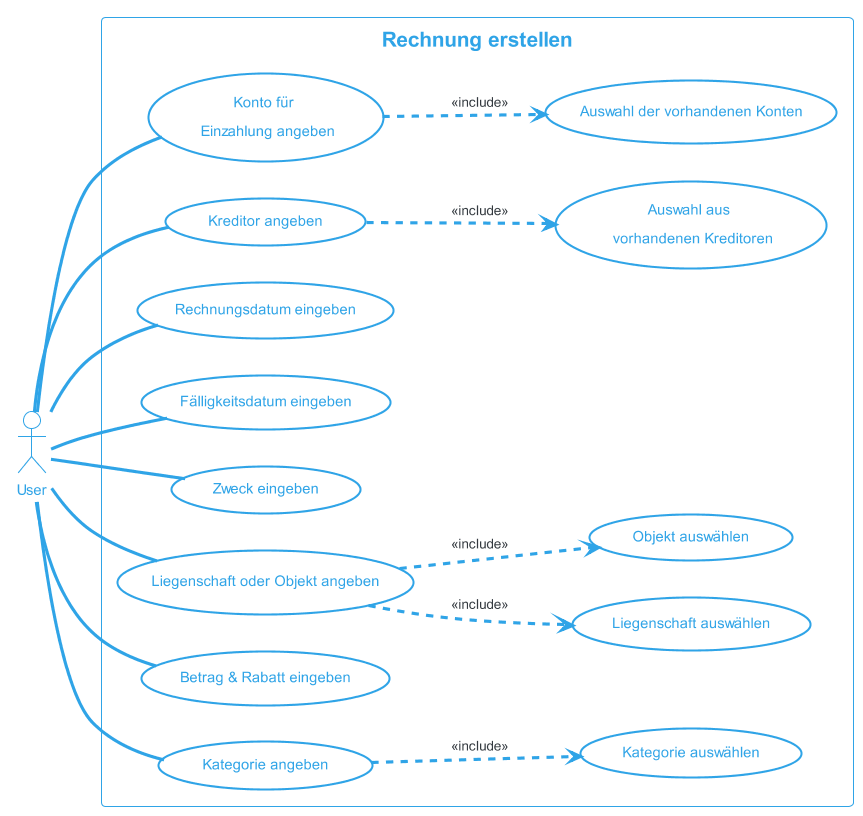
\includegraphics[width=0.8\linewidth]{content/diagrams/out/usecase/rechnungErstellen/Rechnung erstellen.png}
    \caption{UC-Rechnung erstellen}
  \end{center}
  \label{RechnungErstellen}
\end{figure}

\begin{table}[H]
  \newcolumntype{a}{>{\columncolor[HTML]{1EB6FF}}L}
  \centering
  \settowidth\tymin{\textbf{Kurzbeschreibung}}
  \setlength\extrarowheight{2pt}
  \begin{tabulary}{1.0\textwidth}{|a|m{12cm}|}
    \hline
    \textbf{Name}& Login\\
    \hline 
    \textbf{Kurzbeschreibung} & \\
    \hline
    \textbf{Beteiligte Aktoren} & \\
    \hline
    \textbf{Fachverantwortlicher} & \\
    \hline
    \textbf{Referenzen} & \\
    \hline
    \textbf{Vorbedingungen} & \\
    \hline
    \textbf{Nachbedingungen} & \\
    \hline
  \end{tabulary}
  \caption{UC-Login}
\end{table}

\begin{figure}[H]
  \begin{center}
    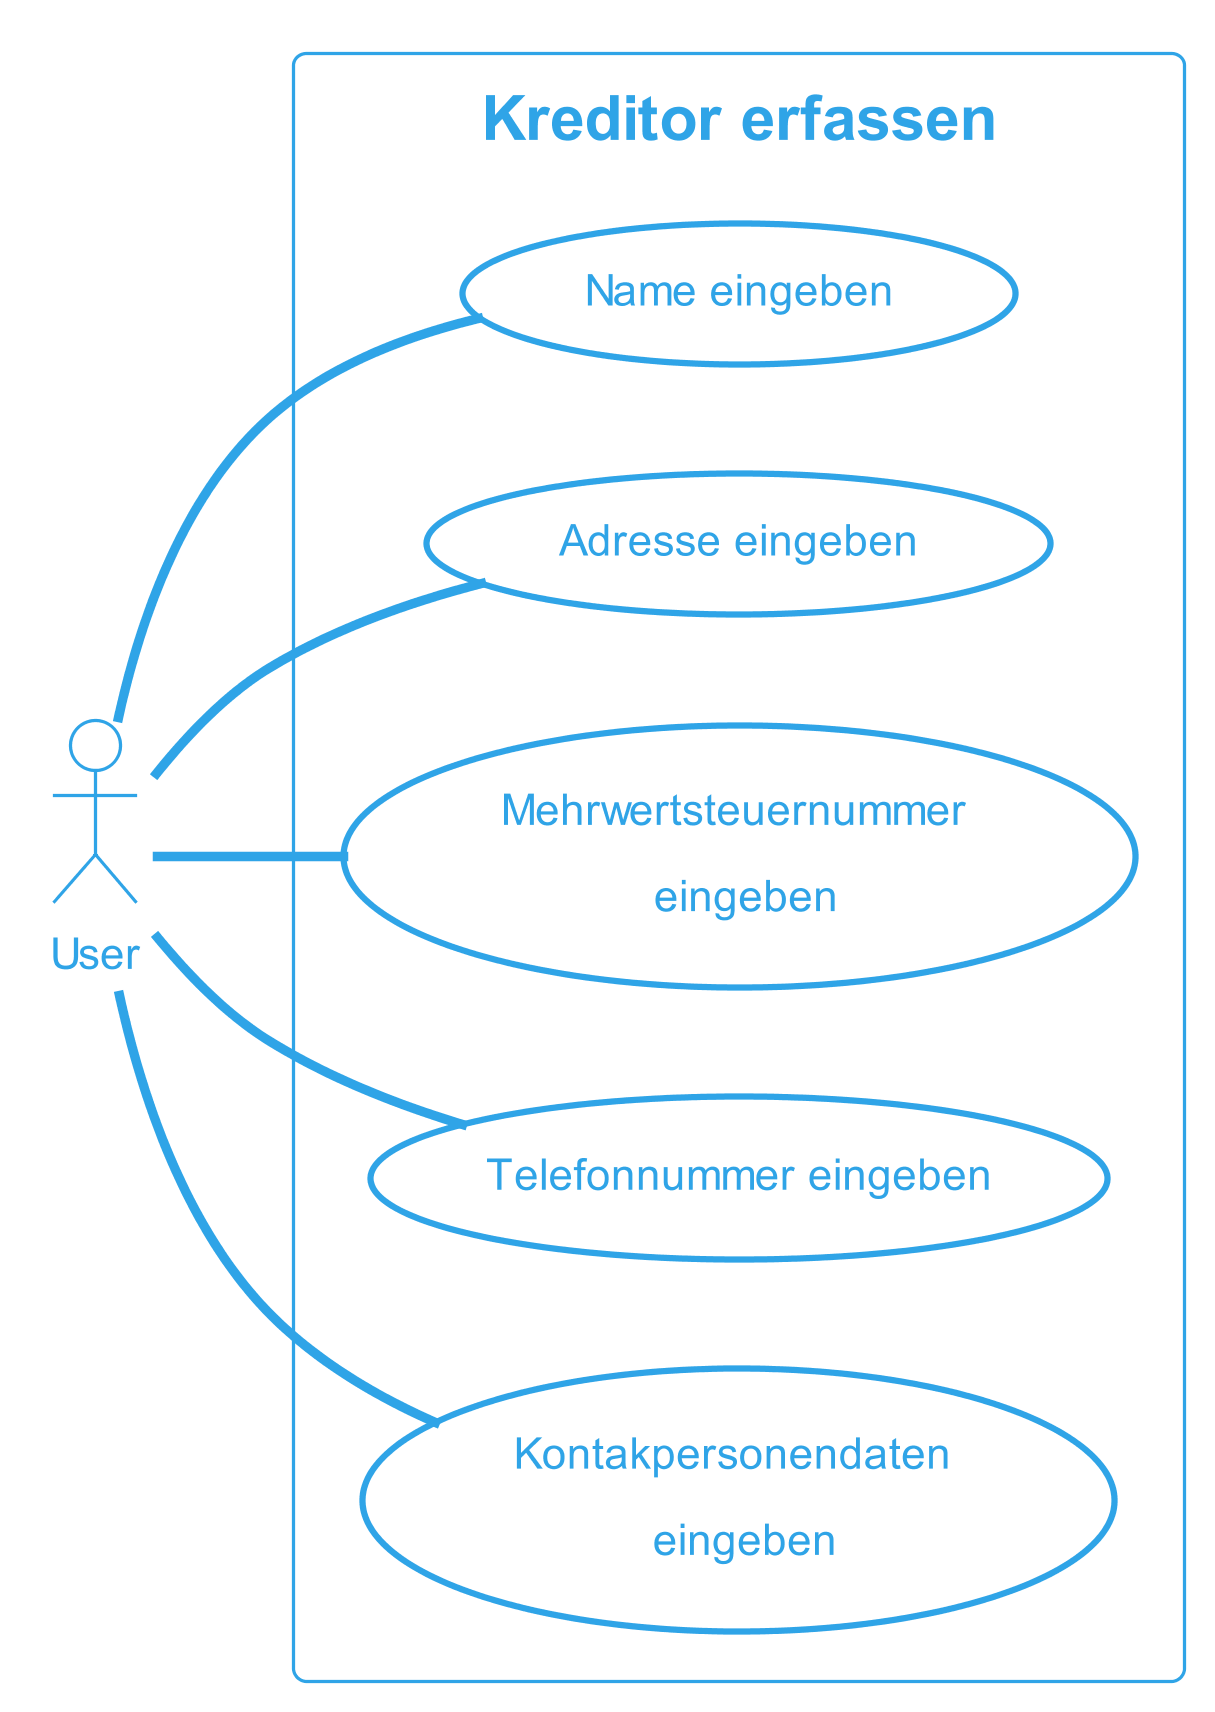
\includegraphics[width=0.4\linewidth]{content/diagrams/out/usecase/kreditorErfassen/Kreditor erfassen.png}
    \caption{UC-Kreditor Erfassen}
  \end{center}
  \label{kreditorErfassen}
\end{figure}

\begin{table}[H]
  \newcolumntype{a}{>{\columncolor[HTML]{1EB6FF}}L}
  \centering
  \settowidth\tymin{\textbf{Kurzbeschreibung}}
  \setlength\extrarowheight{2pt}
  \begin{tabulary}{1.0\textwidth}{|a|m{12cm}|}
    \hline
    \textbf{Name}& Login\\
    \hline 
    \textbf{Kurzbeschreibung} & \\
    \hline
    \textbf{Beteiligte Aktoren} & \\
    \hline
    \textbf{Fachverantwortlicher} & \\
    \hline
    \textbf{Referenzen} & \\
    \hline
    \textbf{Vorbedingungen} & \\
    \hline
    \textbf{Nachbedingungen} & \\
    \hline
  \end{tabulary}
  \caption{UC-Login}
\end{table}

\begin{figure}[H]
  \begin{center}
    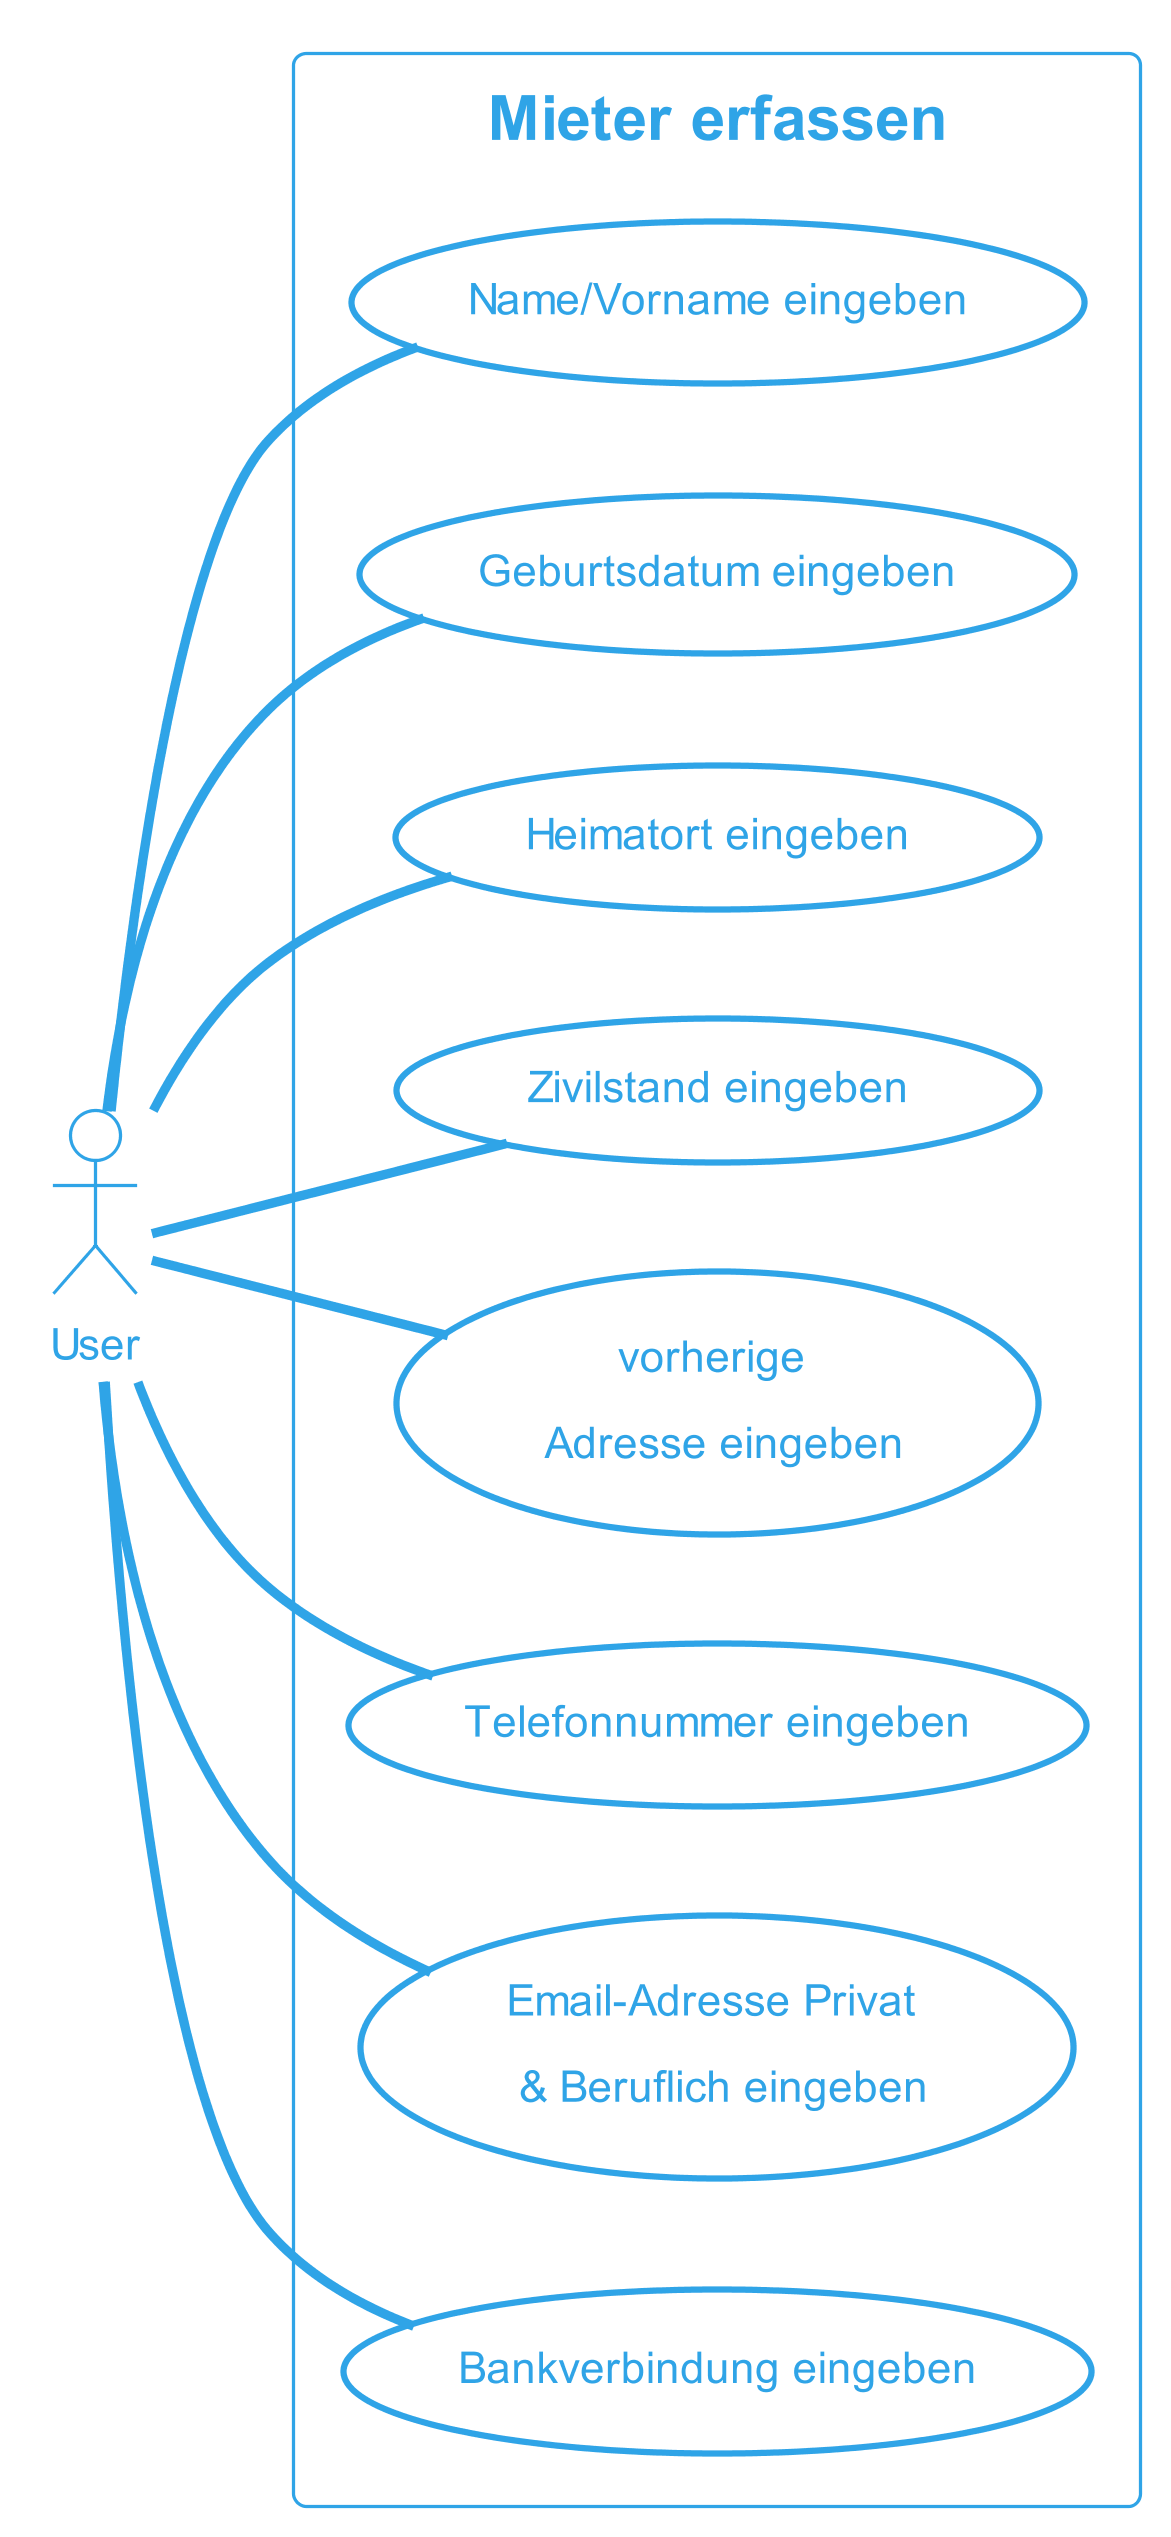
\includegraphics[width=0.4\linewidth]{content/diagrams/out/usecase/mieterErfassen/Mieter erfassen.png}
    \caption{UC-Mieter erfassen}
  \end{center}
  \label{mieterErfassen}
\end{figure}

\begin{table}[H]
  \newcolumntype{a}{>{\columncolor[HTML]{1EB6FF}}L}
  \centering
  \settowidth\tymin{\textbf{Kurzbeschreibung}}
  \setlength\extrarowheight{2pt}
  \begin{tabulary}{1.0\textwidth}{|a|m{12cm}|}
    \hline
    \textbf{Name}& Login\\
    \hline 
    \textbf{Kurzbeschreibung} & \\
    \hline
    \textbf{Beteiligte Aktoren} & \\
    \hline
    \textbf{Fachverantwortlicher} & \\
    \hline
    \textbf{Referenzen} & \\
    \hline
    \textbf{Vorbedingungen} & \\
    \hline
    \textbf{Nachbedingungen} & \\
    \hline
  \end{tabulary}
  \caption{UC-Login}
\end{table}